\chapter{Eye information processes}
This chapter provides an overview of an \gls{eye-process}. I define an eye information process as any process that uses a human eye as its input and has the aim of extracting some property of interest from it. The term thus covers both systems that analyse eye movement, i.e. eye-tracking, and eye appearance, e.g. iris recognition, retinal imagery, etc. 

The first section provides an overview of the anatomy of human eyes. It serves as a reference for easily understanding how eye information processes uses the anatomy for their operation as well as what the physical limitations are. 

Next, the foundations of modern eye-tracking systems will be presented. The goal is to provide the reader with a birds-eye view of the field and its methods.

The final section focuses on sensitive information. Both appearance-based extraction techniques such as iris recognition and gaze-based techniques such as attention-analysis will be presented. 


\section{Anatomy}
Our eyes are an essential part of the human existence. What is so special about the eyes is that they are not just sensory apparatuses for enabling us to register many properties of the physical world around us but also reveal a wealth of information about their owner's current physical and mental state. From a social perspective, eye movements communicate where their owner are looking which typically corresponds with their focus of attention. Additionally, eyes are clearly used socially as indicators of well-being as well as social interaction, i.e. by looking into the eyes of other people. It is likely no coincidence that the eyes have often mythologically been described as doorways to the soul or in some other way been seen as a logical end-point of our minds. To see is often analogous to understand or realise. 

\begin{figure}
    \centering
    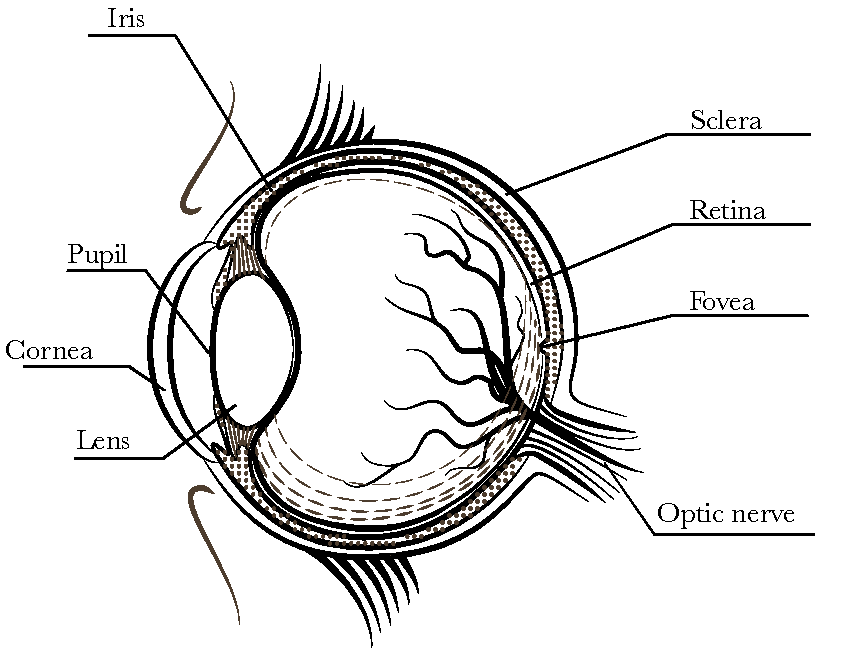
\includegraphics[width=0.8\linewidth]{figures/eye.pdf}
    \caption{Diagram of the human eye. A number of significant features have been marked. Image adapted in accordance with licence from \cite{freepik}.}
    \label{fig:my_label}
\end{figure}

From a physiological perspective, the eye is an incredibly complex organ which reacts in variou...


Figure (REF) shows an overview of a right eye. It is shaped approximately like a sphere with a bulge where the \emph{cornea} is places. The most interesting areas from the perspective of eye information processes, are the retina and the frontal lens complex. 

The \emph{retina} is a tissue covering the inside of the eye. It is composed of light sensitive neurons called photoreceptors, which react to either a wide (rods) or narrow (cones) band of light bandwidths. The rods are used for black/white vision, typically in low-light conditions due to their much higher sensitivity than cones. Cones are primarily used for colour vision as there are three types which each respond to a specific band of wavelengths. Cones have a much higher concentration around a small area on the retina called the \emph{fovea}. This area enables high visual acuity and is therefore generally considered the primary place of attention. In fact, it is well-known that, in spite of the rapid drop-off in photoreceptor density outside the fovea, the human brain succeeds in combining visual information from many individual fixations to produce what seems like high-resolution visual perception.

\begin{figure}
    \centering
    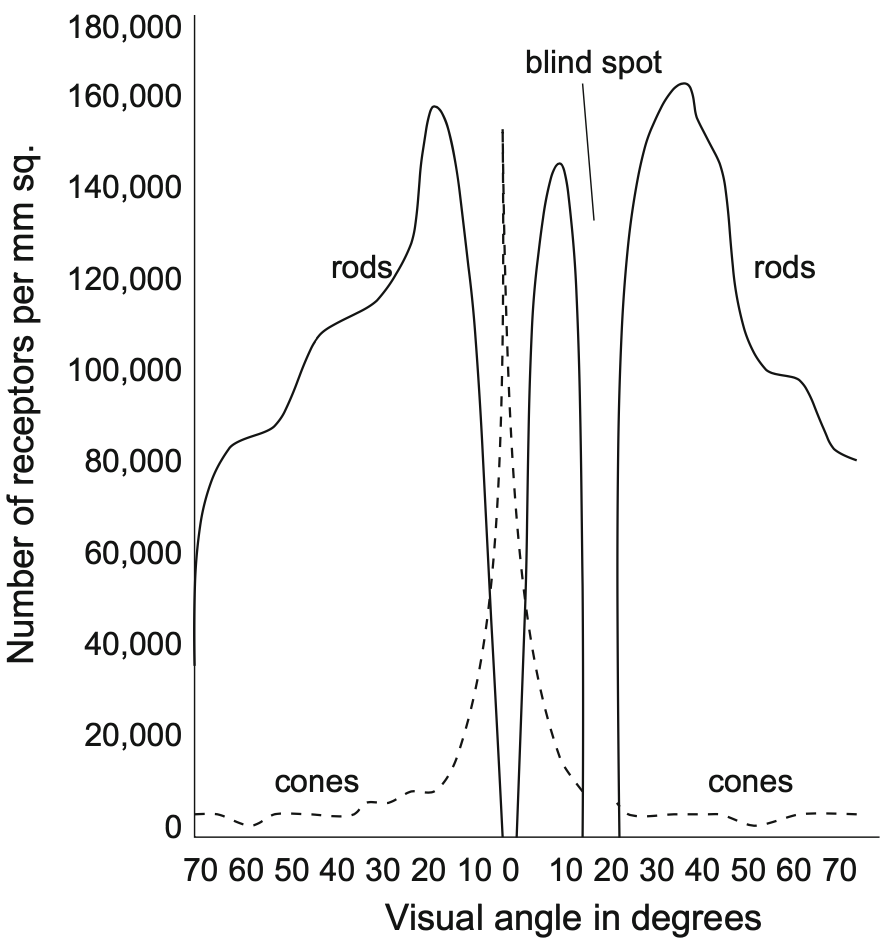
\includegraphics[width=0.6\linewidth]{figures/retina-density.png}
    \caption{Photoreceptor density as a function of visual angle (centred at the fovea). From \parencite{methodology}.}
    \label{fig:my_label}
\end{figure}

The fovea is very important for determining gaze direction or point-of-regard since it determines what is known as the \emph{visual} axis which intersects the lens centre and fovea. This visual axis typically varies slightly (about 5 degrees) from the \emph{optical axis} which intersects the cornea, pupil, and lens. This variation is different from person to person which has to be corrected by an eye-tracker. Typical modern eye-trackers have gaze direction errors of about $0.5^\circ-1.5^\circ$ which is much lower than the $\pm 5^\circ$ of the visual axis.

The frontal lens complex contains the components that allow light to enter the eye in a controlled manner. The lens system is composed of the static \emph{cornea} which accounts for a majority of the eye's optical power and the \emph{lens} which is adjusted by muscles called \emph{ciliary bodies} located behind the iris. The \emph{iris} is composed of muscles that control the size of the circular opening in its middle known as the \emph{pupil}. This allows the eye to adjust the amount of light entering the eye. 

\subsection{Eye movements}
Eye movements are formed of both conscious, semiconscious, and unconscious actions. This has led to great interest in studying these movements for various purposes, including behavioural studies as well as ...

There are five basic categories of eye movements: saccades, vergence movements, smooth pursuits, vestibular, and physiological nystagmus \parencite[39]{methodology}. Saccades are further subdivided into macro- and micro-saccades. Macro-saccades are the typical jerky movements we perform when moving from fixation to fixation. Micro-saccades are involuntary movements of $0.03-2$ degrees. The purpose of micro-saccades is to change the light-stimulus on the retina, since continuous stimulus of photoreceptors results in decreasing activation strength over time \parencite[44]{methodology}. Smooth pursuits are a mode of movement where the eye follows a fixation point on a moving object. Vergence movements are relative movements of the left and right eye to ensure vergence of the visual axes at the point of fixation \parencite{methodology}.


\section{Eye-tracking}
Knowing where people are looking is useful both for studying human behaviour and providing interactive technologies. 

Eye-tracking is a scientific field that cover many different disciplines from computer science and engineering to psychology and biology. These can be divided into the research in eye-tracking technology and research enabled by eye-tracking technology. This section focuses on the former. It gives a short introduction to the eye-tracking technologies available today, how they work, and where they are used.


\section{Privacy}
This section presents potentially sensitive information sources in eye-tracking systems. The first part focuses on sensitive information that is extracted directly from eye images and the second part focuses on information derived from gaze signals.
